\documentclass[notitlepage]{revtex4-1}
% includes...
\usepackage{amsmath}
\usepackage{bm}
\usepackage{natbib}
\usepackage{graphicx}
\usepackage{hyperref}
\usepackage{epstopdf}
\usepackage{color}

\begin{document}
%front matter
\title{A scalable high-order mesh-free framework for direct numerical simulations of combustion}

\author{J. R. C. King}
\email{jack.king@manchester.ac.uk}
\affiliation{Department of Mechanical, Aerospace and Civil Engineering, The University of Manchester, Manchester, M13 9PL, UK}
\date{\today}
\begin{abstract}
This document details the governing equations and numerical methods used in the \textbf{S}calable \textbf{U}nstructured \textbf{N}ode-\textbf{SET} code (aka. SUNSET code).

\end{abstract}

\maketitle
%end front matter

\section{Introduction}

This document describes the \textbf{S}calable \textbf{U}nstructured \textbf{N}ode-\textbf{SET} code (aka. SUNSET code). The code is designed for direct numerical simulations of compressible turbulent reacting flows in complex geometries. It builds on the work in~\cite{king_2020,king_2022}, using the Local Anisotropic Basis Function Method (LABFM) for spatial discretisation, combined with high-order finite differences in the third dimension, and a third-order Runge-Kutta time integration.

Key features:
\begin{itemize}
\item Nearly arbitrary geometries in the $x_{1}-x_{2}$ plane. Homogeneous in the $x_{3}$ direction.
\item High-order ($8^{th}$) discretisation in space dropping to $4^{th}$ order at boundaries.
\item $3^{rd}$ order time integration.
\item NSCBC formulation for (non-reflecting) inflows and outflows, and isothermal or adiabatic walls.
\item Periodic/symmetry boundaries also available.
\item Spatially variable resolution, including on boundaries.
\item Parallelised for MPI+OpenMP, scales well up to $>1000$ cores.
\item Can handle any desired level of chemistry (e.g. single-step, $21$ step $H_{2}$, $25$ step $CH_{4}$)
\end{itemize}


\subsection{A comment on notation}

Subscripts $i$, $j$, and $k$ are vector indices for Einstein notation.
Subscripts $\alpha$ and $\beta$ indicate chemical species.
Subscripts $a$ and $b$ indicate collocation point indices.
Subscripts $l$ and $L$ are used for polynomial coefficient indices.
Subscript $m$ is for chemical reaction number (regular $m$ is polynomial order).

\section{Governing Equations}\label{ge}

The code solves the compressible Navier-Stokes equations in conservative form
\begin{subequations}\begin{align}
\frac{\partial\rho}{\partial{t}}+\frac{\partial\rho{u}_{k}}{\partial{x}_{k}}=&~0\label{eq:mass}\\
\frac{\partial\rho{u}_{i}}{\partial{t}}+\frac{\partial\rho{u}_{i}u_{k}}{\partial{x}_{k}}=&-\frac{\partial{p}}{\partial{x}_{i}}+\frac{\partial\tau_{ki}}{\partial{x}_{k}}+\rho{f}_{i}\label{eq:mom}\\
\frac{\partial\rho{E}}{\partial{t}}+\frac{\partial\rho{u}_{k}E}{\partial{x}_{k}}=&-\frac{\partial{p}u_{k}}{\partial{x}_{k}}-\frac{\partial{q}_{k}}{\partial{x}_{k}}+\frac{\partial\tau_{ki}u_{i}}{\partial{x}_{k}}+\rho\displaystyle\sum_{\alpha}Y_{\alpha}f_{k}\left({u}_{k}-V_{\alpha,k}\right)\label{eq:en}\\
\frac{\partial\rho{Y}_{\alpha}}{\partial{t}}+\frac{\partial\rho{u}_{k}Y_{\alpha}}{\partial{x}_{k}}=&~\dot\omega_{\alpha}-\frac{\partial\rho{V}_{\alpha,k}Y_{\alpha}}{\partial{x}_{k}}\qquad\forall\alpha\in\left[1,N_{S}\right]\label{eq:Y}
\end{align}
\end{subequations}
where $\rho$ is the density, ${u}_{i}$ the $i$-th component velocity, $p$ the pressure, $E$ the total energy, $\tau$ the viscous stress, $f$ a body force, $q$ the heat flux, $Y_{\alpha}$ the concentration of species $\alpha\in\left[1,N_{S}\right]$, and $V_{\alpha,k}$ is the $k$-th component of the molecular diffusion velocity of species $\alpha$. $\dot\omega_{\alpha}$ is the production rate of species $\alpha$.

The viscous stress is defined as 
\begin{equation}\tau_{ki}=\mu\left(\frac{\partial{u}_{k}}{\partial{x}_{i}}+\frac{\partial{u}_{i}}{\partial{x}_{k}}-\frac{2}{3}\frac{\partial{u}_{j}}{\partial{x}_{j}}\delta_{ik}\right)\label{eq:tau},\end{equation}
where $\mu$ is the dynamic viscosity and $\delta_{ik}$ is the Kronecker delta. The energy is
\begin{equation}E=\displaystyle\sum_{\alpha}h_{\alpha}Y_{\alpha}-\frac{p}{\rho}+\frac{1}{2}{u}_{i}{u}_{i}\label{eq:E}\end{equation}
where the sum over $\alpha$ is over all $\alpha\in\left[1,N_{S}\right]$, and $h_{\alpha}$ is the enthalpy of species $\alpha$. The molecular diffusion term in~\eqref{eq:Y} is modelled as a Fickian diffusion process with
\begin{equation}-\rho{V}_{\alpha,k}Y_{\alpha}=\rho\hat{V}_{\alpha,k}Y_{\alpha}-Y_{\alpha}\displaystyle\sum_{\beta\in\left[1,N_{S}\right]}\rho\hat{V}_{\beta,k}Y_{\beta}\label{eq:fickdiff},\end{equation}
in which $\rho\hat{V}_{\alpha,k}Y_{\alpha}$ is obtained from the diffusion model (either constant Lewis numbers or mixtured-averaged), and the final term is a correction to ensure that 
\begin{equation}\displaystyle\sum_{\alpha}Y_{\alpha}=1.\label{eq:sumY}\end{equation}
The heat flux vector is then given by
\begin{equation}q_{k}=-\lambda\frac{\partial{T}}{\partial{x}_{k}}+\displaystyle\sum_{\alpha}\rho{V}_{\alpha,k}Y_{\alpha}h_{\alpha}\label{eq:hfv},\end{equation}
where $\lambda$ is the thermal conductivity of the mixture.
The system is closed with an ideal gas equation of state
\begin{equation}\frac{p}{\rho}={R}_{mix}T=\frac{R_{0}T}{W_{mix}}={R}_{0}T\displaystyle\sum_{\alpha}\frac{Y_{\alpha}}{W_{\alpha}}\label{eq:eos}\end{equation}
where $R_{mix}$ is the gas constant for the mixture, $R_{0}$ is the universal gas constant, and $W_{\alpha}$ is the molar mass of species $\alpha$, and $W_{mix}$ is the molar mass of the mixture.

Reaction rates $\dot\omega_{\alpha}$ are obtained through finite rate chemical kinetics mechanisms - details/refsXX. XX Including Lindemann steps, gibbs backwards rates and third bodies.
Specific heat capacities, enthalpies and gibbs functions are obtained through CHEMKIN/NASA polynomials XXrefXX.

\subsection{Evaluation of temperature and heat capacity}

The temperature dependence of the specific heat capacity of species $\alpha$ is given by a polynomial of order $L$
\begin{equation}c_{p,\alpha}=\displaystyle\sum_{l=1}^{L}a_{\alpha,l}T^{l-1},\end{equation}
which is valid over a specified temperature range $T\in\left[T_{low},T_{high}\right]$, and in which the coefficients $a_{\alpha,l}$ are taken from CHEMKIN tables. Integration of this yields an expression for the enthalpy
\begin{equation}h_{\alpha}=\displaystyle\sum_{l=1}^{L}\frac{a_{\alpha,l}}{l}T^{l} + a_{\alpha,L+1},\end{equation}
whilst the temperature derivative of $c_{p,\alpha}$ is
\begin{equation}\frac{dc_{p,\alpha}}{dT}=\displaystyle\sum_{l=1}^{L}\left(l-1\right)a_{\alpha,l}T^{l-2}.\end{equation}
Noting that the specific heat capacity of species $\alpha$ is $R_{0}/W_{\alpha}$, where $R_{0}$ is the universal gas constant and $W_{\alpha}$ is the molar mass of species $\alpha$, the energy can be written as
\begin{equation}E=\displaystyle\sum_{\alpha}Y_{\alpha}\left(h_{\alpha}-R_{0}\frac{T}{W_{\alpha}}\right)+\frac{1}{2}\bm{u}\cdot\bm{u}.\end{equation}
Substituting the polynomial for $h_{\alpha}$ and collecting terms in powers of $T$, we can write
\begin{equation}f\left(T\right)=C_{0}+\displaystyle\sum_{l=1}^{L}C_{l}T^{l}=0,\label{eq:nonlinearT}\end{equation}
where the coefficients $C$ are given by
\begin{subequations}\begin{align}
C_{0}&=\frac{1}{2}\bm{u}\cdot\bm{u}-E+\displaystyle\sum_{\alpha}Y_{\alpha}a_{\alpha,L+1}\\
C_{1}&=\displaystyle\sum_{\alpha}Y_{\alpha}a_{\alpha,1} - R_{mix}\\
C_{l}&=\displaystyle\sum_{\alpha}Y_{\alpha}\frac{a_{\alpha,l}}{l}\qquad\forall{l}\in\left[2,L\right].\end{align}\end{subequations}
The derivative of $f$ is
\begin{equation}f^{\prime}\left(T\right)=\displaystyle\sum_{l=1}^{L}lC_{l}T^{l-1}.\end{equation}
Having calculated the coefficients $C$, we solve the nonlinear equation~\eqref{eq:nonlinearT} numerically via a Newton-Raphson method to obtain the temperature $T$.

Note that in the case where $a_{\alpha,1}\ne0$ and $a_{\alpha,l\in\left[2,L\right]}=0$ (i.e. $c_{p,\alpha}$ is independent of temperature), $f\left(T\right)$ is linear in $T$, and the Newton-Raphson method will converge (exactly) after a single iteration.

\subsection{Transport properties}

Two models are implemented for transport properties. The constant Lewis number approximation, and a mixture averaged transport model.

\subsubsection{Constant Lewis numbers}

In this model, the diffusive flux is given by
\begin{equation}\rho\hat{V}_{\alpha,k}Y_{\alpha}=-\rho{D}_{\alpha}\frac{\partial{Y}_{\alpha}}{\partial{x}_{k}},\end{equation}
in which $D_{\alpha}$ is the molecular diffusivity of species $\alpha$. The temperature dependence of transport properties is modelled by the relationship
\begin{equation}\mu=\mu_{ref}\left(\frac{T}{T_{ref}}\right)^{r_{T}},\label{eq:tdtp_mu}\end{equation}
where $\mu_{ref}$ is the viscosity at the reference temperature $T_{ref}$, and $r_{T}=0.7$ is a constant exponent. The mixture thermal conductivity is given by
\begin{equation}\lambda=\frac{\mu{c}_{p}}{Pr},\end{equation}
in which $c_{p}$ is the heat capacity of the mixture, and $Pr$ is the Prandtl number, taken as constant. The molecular diffusivity of species $\alpha$ is given by
\begin{equation}D_{\alpha}=\frac{\lambda}{\rho{c}_{p}Le_{\alpha}},\end{equation}
where $Le_{\alpha}$ is the Lewis number for species $\alpha$, which is assumed constant for each species.

\subsubsection{Mixtured-averaged transport}

In this model the diffusive flux is given by 
\begin{equation}\rho\hat{V}_{\alpha,k}Y_{\alpha}=-\rho{D}_{\alpha}\frac{\partial{Y}_{\alpha}}{\partial{x}_{k}}-\rho{D}_{\alpha}Y_{\alpha}\left(\frac{\partial\ln{T}}{\partial{x}_{k}}+\frac{\partial\ln\rho}{\partial{x}_{k}}-\frac{W_{\alpha}}{\rho{R}_{0}T}\frac{\partial{p}}{\partial{x}_{k}}\right),\end{equation}


Chemkin polynomial fits for transport data~\cite{kee_1986}
Review of transport models in~\cite{giacomazzi_2008}.
Mixture-averaged transport for diffusion using Hirschfelder-Curtiss approximation~\cite{hirschfelder_curtiss}.
Combination rule for viscosity and thermal conductivity following~\cite{ern_1994,ern_1995}.

Here the transport properties for individual species and species pairs are evaluated using polynomials [xx ref xx], where
\begin{subequations}\begin{align}
\ln\mu_{\alpha}&=\displaystyle\sum_{l=1}^{L}c_{\mu,\alpha,l}\left(\ln\left(\frac{T}{T_{ref}}\right)\right)^{l-1}\\
\ln\lambda_{\alpha}&=\displaystyle\sum_{l=1}^{L}c_{\lambda,\alpha,l}\left(\ln\left(\frac{T}{T_{ref}}\right)\right)^{l-1}\\
\ln{D}_{\alpha\beta}&=\ln\left(\frac{p_{ref}}{p}\right)+\displaystyle\sum_{lj=1}^{L}c_{D,\alpha\beta,l}\left(\ln\left(\frac{T}{T_{ref}}\right)\right)^{l-1},
\end{align}\end{subequations}
in which the $c_{\dots,l}$ are constants, and $L=4$. [xx more details xx].

The transport properties are then obtained from combination rules as
\begin{equation}\mu=\left[\displaystyle\sum_{\alpha}X_{\alpha}\mu_{\alpha}^{n_{\mu}}\right]^{\frac{1}{n_{\mu}}},\end{equation}
with $n_{\mu}=6$, 
\begin{equation}\lambda=\left[\displaystyle\sum_{\alpha}X_{\alpha}\lambda_{\alpha}^{n_{\lambda}}\right]^{\frac{1}{n_{\lambda}}},\end{equation}
with $n_{\lambda}=1/4$, and
\begin{equation}D_{\alpha}=\frac{\displaystyle\sum_{\beta\ne\alpha}X_{\beta}{W}_{\beta}}{W_{mix}\displaystyle\sum_{\beta\ne\alpha}\frac{X_{\beta}}{D_{\alpha\beta}}}.\end{equation}
Note that the molar concentration $X_{\alpha}=Y_{\alpha}W_{mix}/W_{\alpha}$.
Soret and Dufour effects are neglected.

\subsection{Evaluation of reaction rates}

The reaction mechanism is given by $M$ equations written in the form
\begin{equation}\displaystyle\sum_{\alpha}\nu_{\alpha,m}^{\prime}\mathcal{M}_{\alpha}\rightarrow\displaystyle\sum_{\alpha}\nu_{\alpha,m}^{\prime\prime}\mathcal{M}_{\alpha}\qquad\forall{m}\in\left[1,M\right],\end{equation}
where $\mathcal{M}_{\alpha}$ symbolises the chemical symbol of species $\alpha$, and 
$\nu_{\alpha,m}^{\prime}$ and $\nu_{\alpha,m}^{\prime\prime}$ are the molar stoichiometric coefficients of species $\alpha$ in equation $m$.

The reaction rate of species $\alpha$ is given by
\begin{equation}\omega_{\alpha}=W_{\alpha}\displaystyle\sum_{m=1}^{M}\hat{\omega}_{\alpha,m}\end{equation}
where $\hat{\omega}_{\alpha,m}$ is the molar production rate of species $\alpha$ due to the $m$-th reaction, and $M$ is the total number of reactions. The molar production rates are given by
\begin{equation}\hat{\omega}_{\alpha,m}=\left(\nu^{\prime\prime}_{\alpha,m}-\nu^{\prime}_{\alpha,m}\right)\left[k_{f,m}\left(T\right)\displaystyle\prod_{\beta=1}^{N_{S}}\left(\frac{\rho{Y}_{\beta}}{W_{\beta}}\right)^{\nu^{\prime}_{\beta,m}}-k_{b,m}\left(T\right)\displaystyle\prod_{\beta=1}^{N_{S}}\left(\frac{\rho{Y}_{\beta}}{W_{\beta}}\right)^{\nu^{\prime\prime}_{\beta,m}}\right],\end{equation}
in which $k_{f,m}$ and $k_{b,m}$ are the forward and backward (respectively) rate constants for reaction $m$. The forward rate constant is given by the Arrhenius expression
\begin{equation}k_{f,m}\left(T\right)=A_{m}T^{n_{m}}\exp\left(-\frac{E_{a,m}}{R_{0}T}\right),\end{equation}
with $A_{m}$, $n_{m}$ and $E_{a,m}$ being specified constants representing the pre-exponential factor, the temperature dependence of the pre-exponential factor, and the activation energy.

\subsubsection{Backwards rate constant}

The backwards rate constant is related to the forward rate constant via
\begin{equation}\ln{k}_{b,m}=\ln{k}_{f,m} + \displaystyle\sum_{\alpha}\left(\nu^{\prime\prime}_{\alpha,m}-\nu^{\prime}_{\alpha,m}\right)\left(\frac{\hat{g}_{\alpha}}{R_{0}T}+\ln\left(\frac{P_{0}}{R_{0}}\right)-\ln{T}\right),\end{equation}
in which $P_{0}$ is a reference pressure, and $\hat{g}_{\alpha}$ is the Gibbs function for species $\alpha$, which is given by
\begin{equation}\frac{\hat{g}_{\alpha}}{W_{\alpha}T}=\frac{a_{\alpha,J+1}}{T}-a_{\alpha,1}\ln{T}+\left(a_{\alpha,1}-a_{\alpha,J+2}\right)-\displaystyle\sum_{j=2}^{J}\frac{a_{\alpha,j}}{j\left(j-1\right)}T^{j-1}.\end{equation}

\subsubsection{Third bodies}

For a step $m$ including third bodies $\mathcal{M}$, reaction rates are scaled by the third-body concentration $c_{M,m}$, which is given by
\begin{equation}c_{M,m}=\displaystyle\sum_{\alpha}\eta_{\alpha,m}\frac{\rho{Y}_{\alpha}}{W_{\alpha}},\end{equation}
and $\eta_{\alpha,m}$ are the third-body efficiencies for species $\alpha$ for step $m$.

\subsubsection{Lindemann forms}

Where the Arrhenius form is insufficient to describe the reaction rate, a pressure (partial pressure/concentration) dependancy is introduced, and the forward reaction rate takes the Lindemann form:
\begin{equation}k_{f,m}=k_{\infty,m}\left(\frac{P_{r}}{1+P_{r}}\right)F_{m},\end{equation}
where $F_{m}$ is the Troe fall-off rate, and a constant for steps with Lindemann form. $P_{r}$ is a reduced pressure given by
\begin{equation}P_{r}=\frac{k_{0,m}}{k_{\infty,m}},\end{equation}
$k_{0,m}$ is the Arrhenius rate of the reaction, and $k_{\infty,m}$ is a second Arrhenius rate. Hence for Lindemann steps, in addition to the three Arrhenius coefficients, the constant $F_{m}$ is prescribed, along with the pre-exponential factor, the temperature dependence of the pre-exponential factor and the activation energy for $k_{\infty,m}$. Note that after evaluation of the rate constants for Lindemann steps, the third-body concentration of the step is reset to unity.

\section{Numerical implementation}\label{ni}

The spatial discretisation is based on the Local Anisotropic Basis Function Method (LABFM) in the first two dimensions, and high-order finite differences in the third dimension. LABFM has been detailed and extensively analysed in~\cite{king_2020,king_2022}, and we refer the reader to these works for a complete description.

The domain is discretised in the $x_{1}-x_{2}$ plane with an unstructured point cloud of $N_{12}$ nodes. The discretisation in the third dimension is uniform: there are $N_{3}$ copies of each node in the $x_{1}-x_{2}$ plane, equispaced along the $x_{3}$ axis. Hence, there are a total of $N=N_{12}N_{3}$ nodes in the domain. Each node $a\in\left[1,N\right]$ has position $x_{a,i}$, a distribution lengthscale $s_{a}$, and a computational stencil lengthscale $h_{a}$. $s_{a}$ is the average node spacing around node $a$, and is analagous to the grid spacing in a finite difference scheme. The spacing in $x_{3}$ is denoted $s_{3}$, and is uniform throughout the domain, whilst $s_{a}$ can vary as a function of $x_{1}$ and $x_{2}$. Each node holds the conservative variables $\rho_{a}$, $\rho{u}_{i,a}$, $\rho{E}_{a}$ and $\rho{Y}_{\alpha,a}$. The governing equations are solved on the set of $N$ nodes. 

\begin{figure}
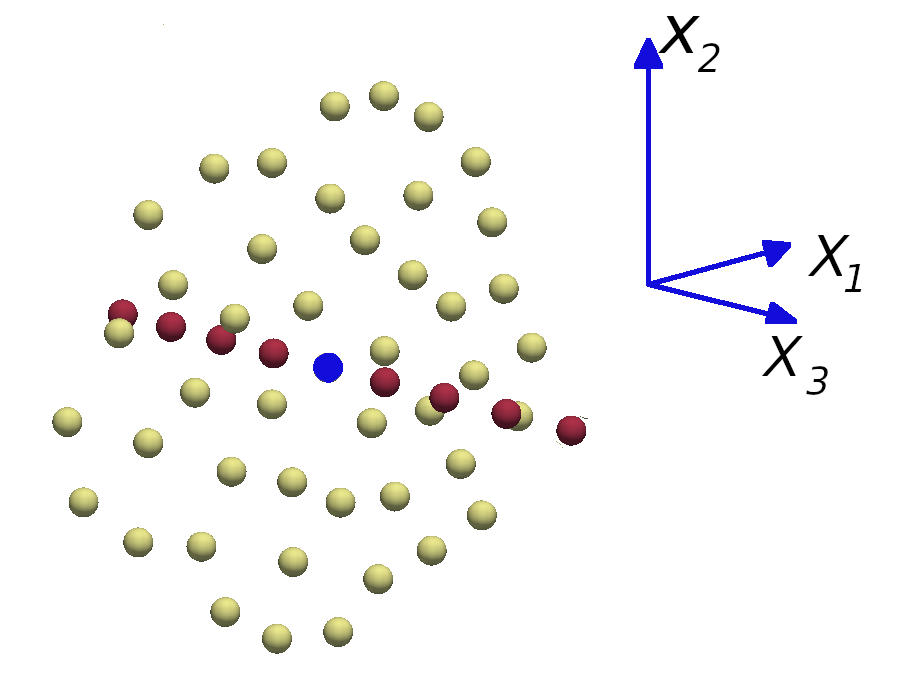
\includegraphics[width=0.6\textwidth]{./stencil.png}
\caption{A typical stencil for a three-dimensional simulation. The nodes shown are those in the stencil of the central node in blue. The unstructured nodes in yellow lie in the same plane (same value of $x_{3}$) as the central node. The nodes in red are those in the finite difference stencil for the $x_{3}$ direction.\label{fig:disc2}}
\end{figure}

The difference between properties at two nodes is denoted $\left(\cdot\right)_{ba}=\left(\cdot\right)_{b}-\left(\cdot\right)_{a}$. The computational stencil for each node $a$ is denoted $\mathcal{N}_{a}$, and is constructed to contain all nodes $b$ in the same $x_{1}-x_{2}$ plane such that $\lvert{x}_{i,ba}x_{i,ba}\rvert\le4h_{a}^{2}$, (with the repeated subscript $i$ implying summation), alongside all the nodes with $x_{1,ba}=x_{2,ba}$ required to build a finite difference stencil in the $x_{3}$ dimension. Figure~\ref{fig:disc2} shows a typical computational stencil.

Figure~\ref{fig:disc1} shows an example discretisation in the present framework for an aerofoil. Wall, inflow and outflow boundaries are discretised with a locally structured node distribution, whilst the remaining space is filled with a quasi-uniform point cloud. XX. The resolution is non-uniform, and in the present example $s$ varies by a factor of $10$ through the domain. The unstructured nodes are created to fill the domain using a variation of the propagating front algorithm of~\cite{fornberg_2015a}, following~\cite{king_2022}.

\begin{figure}
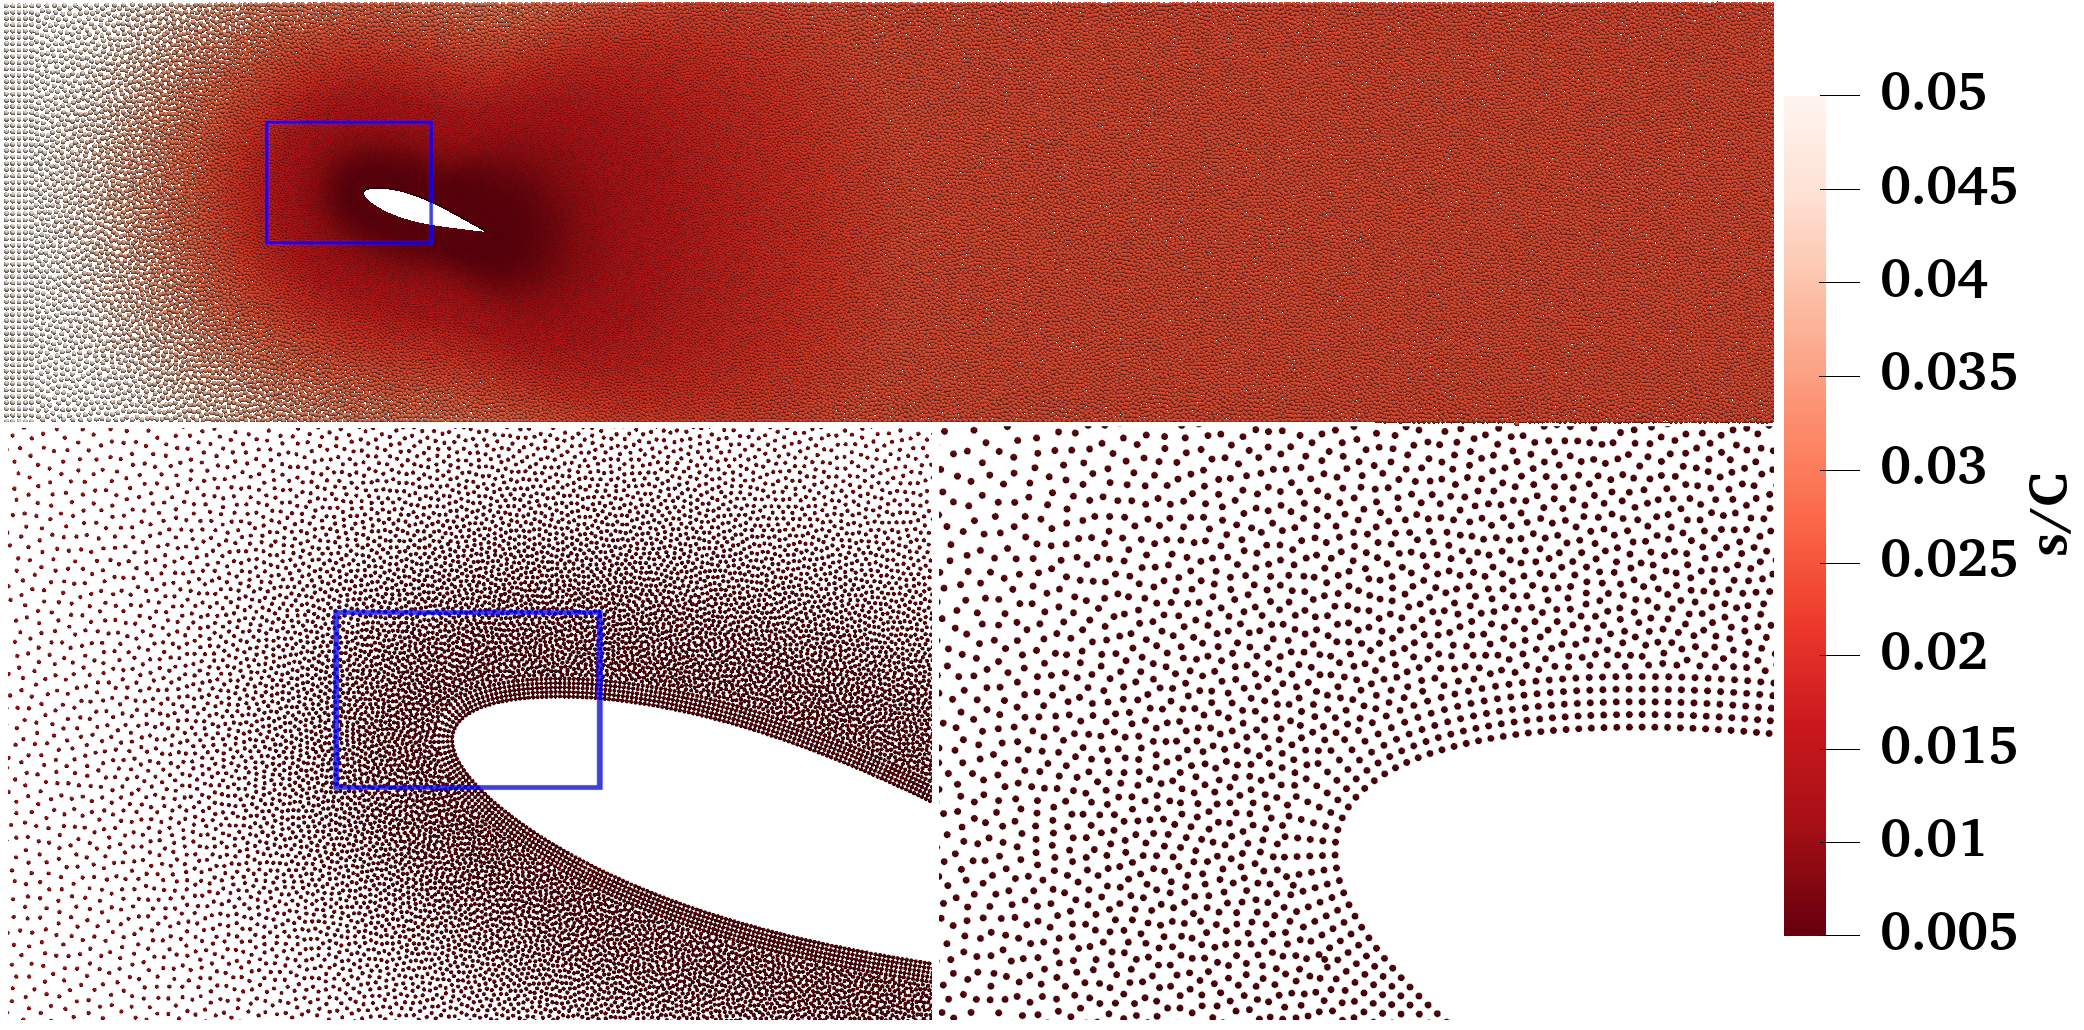
\includegraphics[width=0.99\textwidth]{./aerofoil_dist.png}
\caption{Example of an unstructured node distribution around an aerofoil. The colour represents the local resolution length-scale $s$ normalised by the aerofoil chord length $C$.\label{fig:disc1}}
\end{figure}


\subsection{Evaluation of spatial derivatives}

Spatial derivative operators take the form
\begin{equation}L^{d}_{a}\left(\cdot\right)=\displaystyle\sum_{b}\left(\cdot\right)_{ba}w^{d}_{ba},\label{eq:general_do}\end{equation}
where $d$ identifies the derivative of interest (e.g. $d=x_{1}$ indicates the operator $L^{d}$ approximates $\partial\left(\cdot\right)/\partial{x}_{1}$, and $d=x_{i}x_{i}$ (summation implied) indicates the operator approximates the Laplacian), and $w^{d}_{ba}$ are a set of inter-node weights for the operator. Note that the construction of~\eqref{eq:general_do} takes the same form for both LABFM-based and finite difference-based derivative approximations. For derivatives in the $x_{3}$ dimension, the weights $w^{d}_{ba}$ are simply central finite difference weights of order $m$. For derivatives in the $x_{1}-x_{2}$ plane, LABFM is used to set the $w^{d}_{ba}$, which is constructed from a weighted sum of anisotropic basis functions centred on node $a$. The basis functions used herein are formed from bi-variate Hermite polynomials multiplied by a radial basis function, and the basis function weights are set such that the operator achieves a specified polynomial consistency $m$. Calculation of these weights is done as a pre-processing step, and described in detail in~\cite{king_2022}. 

The order of the spatial discretisation can be specified between $m=4$ and $m=10$, and although there is capability for this to be spatially (or temporally) varying, in this work we set $m=8$ uniformly away from boundaries (except where explicitly stated in our investigations of the effects of changing $m$). This provides a good compromise between accuracy and computational cost. At non-periodic boundaries, the consistency of the LABFM reconstruction is smoothly reduced to $m=4$. The stencil scale $h_{a}$ is initialised to $h_{a}=2.7s_{a}$ in the bulk of the domain, and $h_{a}=2.4s_{a}$ near boundaries (choices informed through experience as being large enough to ensure stability). In bulk of the domain, the stencil scale is then reduced following the optimisation procedure described in~\cite{king_2022}. This has the effect of both reducing computational costs, and increasing the resolving power of LABFM, yielding the smallest stencil size $h_{a}$ for which the discretisation remains stable.

The evaluation of derivatives using~\eqref{eq:general_do} constitutes the bulk of the computational cost, and it is hence desirable only use it where essential, and where possible to use analytic expressions to relate derivatives of secondary properties to those evaluated via~\eqref{eq:general_do}. First derivatives of $\rho$, ${u}_{i}$, $\rho{E}$ and ${Y}_{\alpha}$, alongside the temperature $T$ and pressure $p$, are evaluated directly using~\eqref{eq:general_do}. Convective terms are then constructed from combinations thereof: for example
\begin{equation}\frac{\partial\rho{u}_{i}E}{\partial{x}_{i}}=u_{i}\frac{\partial\rho{E}}{\partial{x}_{i}}+\rho{E}\frac{\partial{u}_{i}}{\partial{x}_{i}}.\end{equation}
Laplacians and direct second (i.e. $\partial^{2}\left(\cdot\right)/\partial{x}_{i}\partial{x}_{i}$) derivatives are also evaluated with~\eqref{eq:general_do}. To avoid the explicit evaluation of cross-second derivatives of velocity, the viscous stress divergence is evaluated as
\begin{equation}\frac{\partial\tau_{ki}}{\partial{x}_{k}}=\frac{1}{\mu}\frac{\partial\mu}{\partial{x}_{k}}\tau_{ki}+\mu\left(\frac{\partial^{2}{u}_{i}}{\partial{x}_{k}\partial{x}_{k}}+\frac{1}{3}\frac{\partial^{2}{u}_{k}}{\partial{x}_{i}\partial{x}_{k}}\right)\label{eq:divtau},\end{equation}
where the final term is the gradient of the velocity divergence, which is calculated through two iterations of first derivative evalations with~\eqref{eq:general_do}. The benefit of this approach is that it reduces the stencil size, and provides a significant reduction in the complexity associated with parallelising the scheme. Gradients of secondary properties are evaluated from analytic expressions in terms of gradients of primary properties. The gradient of the enthalpy of species $\alpha$ is given by
\begin{equation}\frac{\partial{h}_{\alpha}}{\partial{x}_{k}}=\frac{dh_{\alpha}}{dT}\frac{\partial{T}}{\partial{x}_{k}}=c_{p,\alpha}\frac{\partial{T}}{\partial{x}_{k}},\end{equation}
and the gradient of the mixture specific heat capacity is
\begin{equation}\frac{\partial{c}_{p}}{\partial{x}_{k}}=\displaystyle\sum_{\alpha}\left[Y_{\alpha}\frac{dc_{p,\alpha}}{dT}\frac{\partial{T}}{\partial{x}_{k}}+c_{p,\alpha}\frac{\partial{Y}_{\alpha}}{\partial{x}_{k}}\right].\end{equation}
When constant Lewis numbers are assumed, additional relations are available to evaluate the spatial derivatives of transport properties:
\begin{equation}\frac{\partial\mu}{\partial{x}_{k}}=\frac{r_{T}\mu}{T}\frac{\partial{T}}{\partial{x}_{k}}\end{equation}
\begin{equation}\frac{\partial\lambda}{\partial{x}_{k}}=\frac{r_{T}\lambda}{T}\frac{\partial{T}}{\partial{x}_{k}}+\frac{\lambda}{c_{p}}\frac{\partial{c_{p}}}{\partial{x}_{k}}\end{equation}
\begin{equation}\frac{\partial\rho{D}_{\alpha}}{\partial{x}_{k}}=\frac{r_{T}D_{\alpha}}{T}\frac{\partial{T}}{\partial{x}_{k}}.\end{equation}
For the mixture averaged model, gradients of $\mu$, $\lambda$ and $\rho{D}_{\alpha}$ are obtained directly using~\eqref{eq:general_do}.

\subsection{Temporal integration and filtering}

The governing equations are integrated in time using a four-step third-order, low-storage explicit Runge-Kutta scheme, with embedded second order error estimation, denoted RK3(2)4[2R+]C in the classification system of~\citet{kennedy_2000}. The value of the time step is set adaptively using a PID controller to keep time-integration errors below a specified threshold (set to $10^{-4}$ in throughout the present work). 

The solution is de-aliased after each time-step by high-order spatial filtering using the filters described in~\cite{king_2022} combined with a finite difference filter following~\cite{kennedy_1994}. 
The combined filter is defined by
\begin{equation}F\left(\phi\right)=-\left(-1\right)^{m/2}\left(\frac{s_{3}}{2}\right)^{m}\frac{\partial^{m}}{\partial{x}_{3}^{m}}\left[\left(1+\kappa_{m}\nabla_{x_{1}x_{2}}^{m}\right)\phi\right]\label{eq:filt},\end{equation}
where $\kappa_{m}$ is the filter coefficient, specific to each node, calculated as in~\cite{king_2022}, and $\nabla_{x_{1}x_{2}}^{m}$ is the two-dimensional Laplacian raised to the power of $m/2$ (as used in the filtering in~\cite{king_2022}), defined in index notation as
\begin{equation}\nabla_{x_{1}x_{2}}^{m}=\displaystyle\sum_{n=0}^{m}{m\choose n}\frac{\partial^{m}}{\partial{x}_{1}^{m-n}\partial{x}_{2}^{n}}.\end{equation}
The term within the square brackets in~\eqref{eq:filt} is the two-dimensional filter in the $x_{1}-x_{2}$ plane, whilst the operator outside the square brackets is the filter in the $x_{3}$ dimension. The filters are applied sequentially in this manner because the filter does not include any cross-components in $x_{1}x_{3}$ or $x_{2}x_{3}$. This approach follows those used in finite difference codes, where the dimensions are filtered sequentially. With the LABFM filter, the $x_{1}$ and $x_{2}$ dimensions are filtered simultaneously, because the filter includes cross-derivative terms.

For density, momenta and energy, we simply apply the filter as defined by~\eqref{eq:filt}, such that the filtered variables passed to the next time step are
\begin{equation}\widetilde{\phi}=F\left(\phi\right)\qquad\text{for}\quad\phi=\rho,\rho{u}_{i},\rho{E}\end{equation}

As with the molecular diffusion terms, the filtering procedure does not guarantee satisfaction of the compatibility criteria~\eqref{eq:sumY}. Hence, we introduce a new correction to the filtering procedure for the species mass fractions, which takes inspiration from the the diffusion correction velocity. We modify the procedure with the addition of a filter correction term $F_{c}$ such that
\begin{equation}\widetilde{\rho{Y}_{\alpha}}=F\left(\rho{Y}_{\alpha}\right)+F_{c},\end{equation}
where 
\begin{equation}F_{c}=\frac{1}{N_{S}}\left[\widetilde{\rho}-\displaystyle\sum_{\alpha}F\left(\rho{Y}_{\alpha}\right)\right]\end{equation}
This approach ensures that
\begin{equation}\displaystyle\sum_{\alpha}\widetilde{Y}_{\alpha}=1\label{eq:filtsumY}\end{equation}
by construction. This method results in the maximum error in~\eqref{eq:filtsumY} remaining below machine precision. In all our simulations, the maximum error in~\eqref{eq:filtsumY} is below $3\times{10}^{-18}$.


\subsection{Boundaries}

The boundary framework largely follows that described in detail for isothermal flows in~\cite{king_2022}, extended to accommodate thermal and reacting flows. The discretisations on boundaries are detailed in Table~\ref{tab:boundaries}. At wall, inflow and outflow boundaries, the node-set is structured, with a band of $5$ rows of uniformly spaced nodes. Wall boundaries may be curved, and the resolution along boundaries need not be uniform. On boundaries, normal derivatives are calculated using one-sided $5$-point finite difference stencils, whilst tangential (in the $x_{1}-x_{2}$ plane) derivatives are obtained with a one-dimensional formulation of LABFM detailed in~\cite{king_2022} with $m=6$. For the first row in from the boundaries (Row $1$), first derivatives are evaluated using asymmetric finite differences (normal) and one-dimensional LABFM (tangential), whilst second derivatives and filters are obtained from two-dimensional LABFM with $m=4$. For nodes in row $2$, all operators use two-dimensional LABFM with $m=4$. For rows $3$ and $4$, all operators use two-dimensional LABFM with $m=6$. Note that at all nodes including boundary nodes, all operators in the third dimension use central finite differences.

\begin{table}
\begin{center}
\caption{Schemes for derivatives near boundaries.\label{tab:boundaries}}
\begin{tabular}{|l|c|c|c|c||}
\hline
\textbf{Node} & Boundary normal derivative & Boundary tangential derivative (in $x_{1}-x_{2}$ plane) & Second derivatives & Filtering operator \\
\hline
Boundary & One-sided FD & 1D-LABFM & FD + 1D-LABFM & FD + 1D-LABFM \\
Row $1$ & Asymmetric FD & 1D-LABFM & LABFM ($m=4$) & LABFM ($m=4$) \\
Row $2$ & LABFM ($m=4$) & LABFM ($m=4$) & LABFM ($m=4$) & LABFM ($m=4$) \\
Row $3$ & LABFM ($m=6$) & LABFM ($m=6$) & LABFM ($m=6$) & LABFM ($m=6$)  \\
Row $4$ & LABFM ($m=6$) & LABFM ($m=6$) & LABFM ($m=6$) & LABFM ($m=6$) \\
\hline
\end{tabular}
\end{center}
\end{table}

Symmetry and periodic boundary conditions are available, alongside no-slip wall boundaries (isothermal or adiabatic), inflows (both partially non-relfecting and ``hard''), non-reflecting outflows. Walls, inflows and outflows are imposed through the Navier Stokes characteristic boundary condition (NSCBC) formalism, following~\cite{sutherland_2003}. The improved outflow conditions of~\cite{yoo_2007} has been implemented, but was found to be less stable to the passage of flames than the method of~\cite{sutherland_2003}.


\subsection{Parallelisation}

The code is accelerated with a shared-distributed framework, using both OpenMP and MPI. A non-uniform block-structured three-dimensional domain decomposition scheme is used, with the physical sizes of subdomains set such that each MPI rank contains the same number of nodes. The decomposition takes as input the desired number of processors in each dimension $N_{P1}$, $N_{P2}$, and $N_{P3}$, giving a total of $N_{P}=N_{P1}N_{P2}N_{P3}$ processors. The allocation of nodes to processors then forms a preprocessing step, following the algorithm:
\begin{enumerate}
\item Generate the node discretisation in the $x_{1}-x_{2}$ plane.
\item Re-arrange the nodes in order of increasing $x_{1}$.
\item Split the discretisation into $N_{P1}$ slice each containing the same number of nodes.
\item For each slice
\begin{enumerate}
\item Re-arrange the nodes in order of increasing $x_{2}$.
\item Split the slice into $N_{P2}$ blocks each containing the same number of nodes.
\item For each slice, create the $x_{3}$ discretisation by creating $N_{3}$ copies equispaced along the $x_{3}$ axis, and split into $N_{P3}$ processor domains.
\end{enumerate}
\end{enumerate}
This approach results in each processor containing the same number of nodes, and load balancing is typically achieved to within $5\%$. 

\appendix
\section{Equations written out in full, in Einstein notation}\label{fulleqns}

The following is valid for constant Lewis numbers. For mixtured-averaged diffusion, there are even more terms in the energy and species equations.

\begin{equation}\frac{\partial\rho}{\partial{t}}+\frac{\partial\rho{u}_{i}}{\partial{x}_{i}}=0\end{equation}

\begin{equation}\frac{\partial\rho{u}_{i}}{\partial{t}}+\rho{u}_{j}\frac{\partial{u}_{i}}{\partial{x}_{j}}+u_{i}\frac{\partial\rho{u}_{j}}{\partial{x}_{j}}=-\frac{\partial{p}}{\partial{x}_{i}}+\mu\left[\frac{\partial^{2}u_{i}}{\partial{x}_{j}\partial{x}_{j}}-\frac{1}{3}\frac{\partial}{\partial{x}_{i}}\left(\frac{\partial{u}_{j}}{\partial{x}_{j}}\right)\right]+\left[\frac{\partial{u}_{i}}{\partial{x}_{j}}+\frac{\partial{u}_{j}}{\partial{x}_{i}}-\frac{2}{3}\delta_{ij}\frac{\partial{u}_{k}}{\partial{x}_{k}}\right]\frac{\partial\mu}{\partial{x}_{j}}+\rho{f}_{i}\end{equation}


\begin{eqnarray}
\frac{\partial\rho{E}}{\partial{t}}+u_{i}\frac{\partial\rho{E}}{\partial{x}_{i}}=&-&\rho{E}\frac{\partial{u}_{i}}{\partial{x}_{i}}-u_{i}\frac{\partial{p}}{\partial{x}_{i}}-p\frac{\partial{u}_{i}}{\partial{x}_{i}}\\
&+&u_{i}\left\{\frac{\mu}{\rho}\left[\frac{\partial^{2}u_{i}}{\partial{x}_{j}\partial{x}_{j}}-\frac{1}{3}\frac{\partial}{\partial{x}_{i}}\left(\frac{\partial{u}_{j}}{\partial{x}_{j}}\right)\right]+\frac{1}{\rho}\left[\frac{\partial{u}_{i}}{\partial{x}_{j}}+\frac{\partial{u}_{j}}{\partial{x}_{i}}-\frac{2}{3}\delta_{ij}\frac{\partial{u}_{k}}{\partial{x}_{k}}\right]\frac{\partial\mu}{\partial{x}_{j}}\right\}\\
&+&\mu\left(\frac{\partial{u}_{i}}{\partial{x}_{j}}+\frac{\partial{u}_{j}}{\partial{x}_{i}}-\frac{2}{3}\delta_{ij}\frac{\partial{u}_{k}}{\partial{x}_{k}}\right)\frac{\partial{u}_{i}}{\partial{x}_{j}}\\
&+&\lambda\frac{\partial^{2}{T}}{\partial{x}_{k}\partial{x}_{k}}+\frac{\partial\lambda}{\partial{x}_{k}}\frac{\partial{T}}{\partial{x}_{k}}\\
&+&\displaystyle\sum_{\alpha}\left\{\rho{D}_{\alpha}\frac{\partial{Y}_{\alpha}}{\partial{x}_{i}}\frac{\partial{h}_{\alpha}}{\partial{x}_{i}}+{h}_{\alpha}\left[\rho{D}_{\alpha}\frac{\partial^{2}Y_{\alpha}}{\partial{x}_{i}\partial{x}_{i}}
+\frac{\partial\rho{D}_{\alpha}}{\partial{x}_{i}}\frac{\partial{Y}_{\alpha}}{\partial{x}_{i}}\right]\right\}\\
&-&\displaystyle\sum_{\alpha}{Y}_{\alpha}h_{\alpha}\displaystyle\sum_{\beta}\left[\rho{D}_{\beta}\frac{\partial^{2}{Y}_{\beta}}{\partial{x}_{i}\partial{x}_{i}}+\frac{\partial\rho{D}_{\beta}}{\partial{x}_{i}}\frac{\partial{Y}_{\beta}}{\partial{x}_{i}}\right]\\
&-&\displaystyle\sum_{\alpha}\left[h_{\alpha}\frac{\partial{Y}_{\alpha}}{\partial{x}_{i}}+Y_{\alpha}\frac{\partial{h}_{\alpha}}{\partial{x}_{i}}\right]\displaystyle\sum_{\beta}\rho{D}_{\beta}\frac{\partial{Y}_{\beta}}{\partial{x}_{i}}\\
&+&\rho\displaystyle\sum_{\alpha}Y_{\alpha}f_{i}\left({u}_{i}-V_{\alpha,i}\right)
\end{eqnarray}
and
\begin{eqnarray}
\frac{\partial\rho{Y}_{\alpha}}{\partial{t}}+\rho{u}_{i}\frac{{Y}_{\alpha}}{\partial{x}_{i}}+Y_{\alpha}\frac{\partial\rho{u}_{i}}{\partial{x}_{i}}=&&\dot\omega_{\alpha}
+\left[\rho{D}_{\alpha}\frac{\partial^{2}Y_{\alpha}}{\partial{x}_{i}\partial{x}_{i}}+\frac{\partial{\rho{D}}_{\alpha}}{\partial{x}_{i}}\frac{\partial{Y}_{\alpha}}{\partial{x}_{i}}\right]\\
&-&Y_{\alpha}\displaystyle\sum_{\beta}\left[\rho{D}_{\beta}\frac{\partial^{2}Y_{\beta}}{\partial{x}_{i}\partial{x}_{i}}+\frac{\partial\rho{D}_{\beta}}{\partial{x}_{i}}\frac{\partial{Y}_{\beta}}{\partial{x}_{i}}\right]-\frac{\partial{Y}_{\alpha}}{\partial{x}_{i}}\displaystyle\sum_{\beta}\rho{D}_{\beta}\frac{\partial{Y}_{\beta}}{\partial{x}_{i}}
\end{eqnarray}

Note, I haven't expanded out $V_{\alpha,i}$ in the body force term in the energy equation in full.



\bibliographystyle{elsarticle-num-names}
\bibliography{jrckbib}

\end{document}


